\begin{scanpage}{0063}{46}
The resulting equations show that in the region $R\gg ka^2$, $ka\sin\theta\gg1$ the fringing field may be investigated as the sum of the spherical waves from two ``luminous'' points on the rim of the disk, the polar angles of which respectively equal $\psi=\phi$ and $\psi=\pi+\phi$. It is not difficult to see that these waves satisfy the Fermi principle. Actually, of all the points on the disk's surface, the point $\rho=a$, $\psi=\phi$ is the closest to the observation point $(R,\theta,\phi)$, and the point $\rho=a$, $\psi=\pi+\phi$ is the furthest from it.

However, Equations (7.13) describe the radiation not only from the two ``luminous'' points, but they determine the field radiated by the entire ``luminous'' region which is adjacent to the line connecting the points $\rho=a$, $\psi=\phi$ and $\rho=a$, $\psi=\pi+\phi$.

Let us show that the luminous region actually makes the main contribution to the fringing field. For this purpose, let us calculate the field radiated by the currents which flow inside the sector encompassing the line $\psi=\phi$ (Figure 18). Let us take the angular dimensions of the sector in such a way that its arc, which equals $2a\Phi_0$, would occupy the first Fresnel zone. When this is done, the angle $\Phi_0$ will satisfy the equation
\par\noindent\begin{minipage}[t]{.45\linewidth}\vspace{0pt}\centering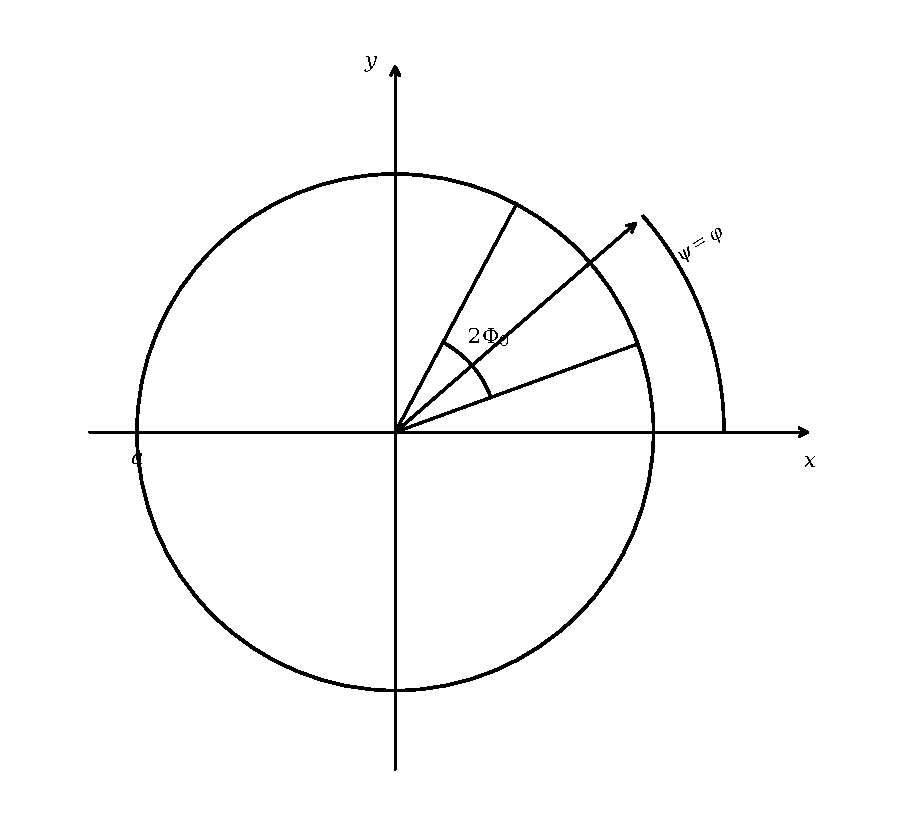
\includegraphics[width=.9\linewidth]{images/recreated/a-0063-fig18.pdf}\par Figure 18. Calculation of the field radiated by the ``luminous'' region of the disk.\end{minipage}\hfill\begin{minipage}[t]{.51\linewidth}\vspace{0pt}
\[a(1-\cos\Phi_0)\sin\theta=\frac\lambda4.\tag{7.14}\]
In the case being investigated by us, when the condition $ka\sin\theta\gg1$ is fulfilled, we have from Equation (7.14)
\[\cos\Phi_0=1-\frac\lambda{4a\sin\theta}\approx1-\frac{\Phi_0^2}2,\tag{7.15}\]
hence
\[\Phi_0=\sqrt{\frac\pi{ka\sin\theta}}.\tag{7.16}\]
\end{minipage}
\end{scanpage}
